\begin{frame}
    \frametitle{Particle Filter}
    \note{Content from Cyrill Stachniss's video: https://youtu.be/MsYlueVDLI0}
    \footnotesize
    \begin{itemize}
        \item With EKF, we are restricted to Gaussian distributions.
        \item When using EKF, we obtain a Gaussian distribution that describes where the robot is located.
        \item In Particle Filter, we use particles or hypotheses that describe where the robot could be.
        \item Instead of having a parametric form like EKF, which describes the probability distribution with the parameters mean $\mu$ and covariance $\covariance$, Partible Filter uses non-parametric samples as hypotheses about where the robot could be.
        \end{itemize}
    
    \begin{center}
        \movie[loop]{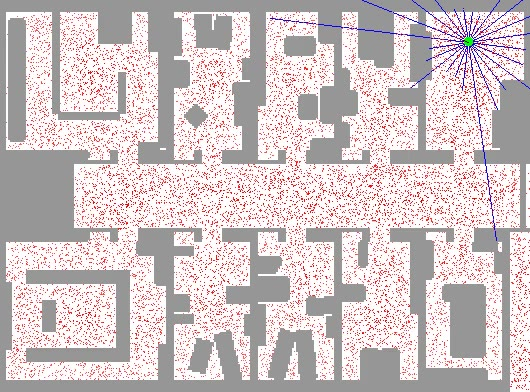
\includegraphics[width=0.4\columnwidth]{images/particle_filter/particle_filter_video.jpg}}{videos/particle_filter.mp4}
    \end{center}
    
    \note{Video from https://rse-lab.cs.washington.edu/projects/mcl/animations/global-floor.gif}
\end{frame}

\begin{frame}
    \frametitle{Flexible Function Approximation}
    \note{Content from Cyrill Stachniss's video: https://youtu.be/MsYlueVDLI0}
    \footnotesize
    
    \begin{itemize}
        \item Goal: Approach that allows estimating any \textbf{arbitrary probability distribution}
    \end{itemize}
    
    \begin{center}
        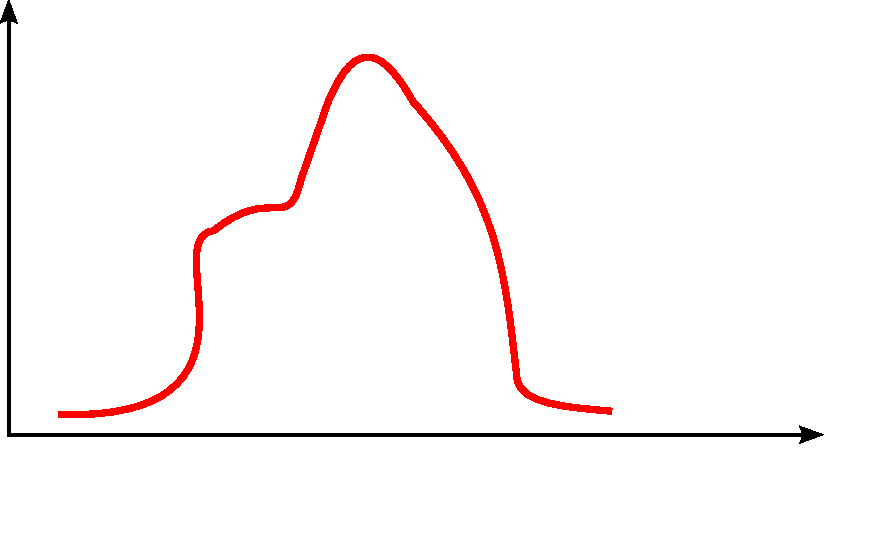
\includegraphics[width=0.5\columnwidth]{./images/particle_filter/arbitrary_distribution.pdf}
    \end{center}

\end{frame}

\begin{frame}
    \frametitle{Using Samples (Particles)}
    \note{Content from Cyrill Stachniss's video: https://youtu.be/MsYlueVDLI0}
    \footnotesize
    \begin{itemize}
        \item \textbf{Multiple samples} to represent an arbitrary probability distribution
        \item The samples are more clustered in some areas and less so in others. The number of particles per unit area describes how likely it is that the robot is in that area.
        \item Each sample accumulates a bit of "probability mass."
        \item The sample can be thought of as an approximation to the probability density function (pdf).
        \item To obtain the pdf, you have to integrate over a certain area to obtain the probability mass of the robot being in that area.
        \item Therefore, where the pdf is high, we will have more particles, and where the pdf is low, we will have fewer particles.
    \end{itemize}
    
    \begin{center}
        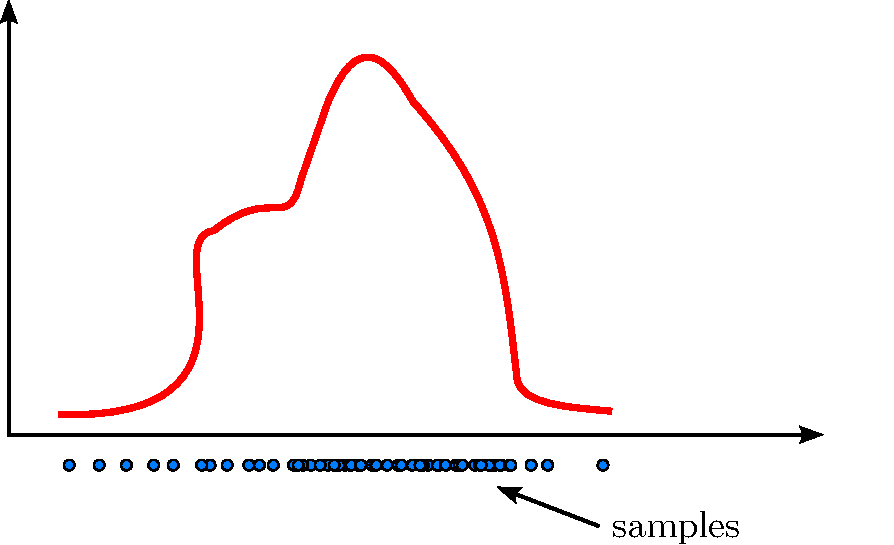
\includegraphics[width=0.4\columnwidth]{./images/particle_filter/arbitrary_distribution_samples.pdf}
    \end{center}

\end{frame}

\begin{frame}
    \frametitle{Using Weighted Samples}
    \note{Content from Cyrill Stachniss's video: https://youtu.be/MsYlueVDLI0}
    \footnotesize
    \begin{itemize}
        \item Instead of using sample accumulation to represent an arbitrary probability distribution, we can use \textbf{Multiple Weighted Samples}
        \item We can reduce the number of samples we need by adding weights to each sample.
        \item The more weight a sample has, the more probability mass there is in that region.
        \item The weights of all the samples together should sum to 1.
        \item Initially, we could add a uniform weight to each sample. For example, if we have $n$ samples, then each sample has weight $\frac{1}{n}$
    \end{itemize}
    
    \begin{center}
        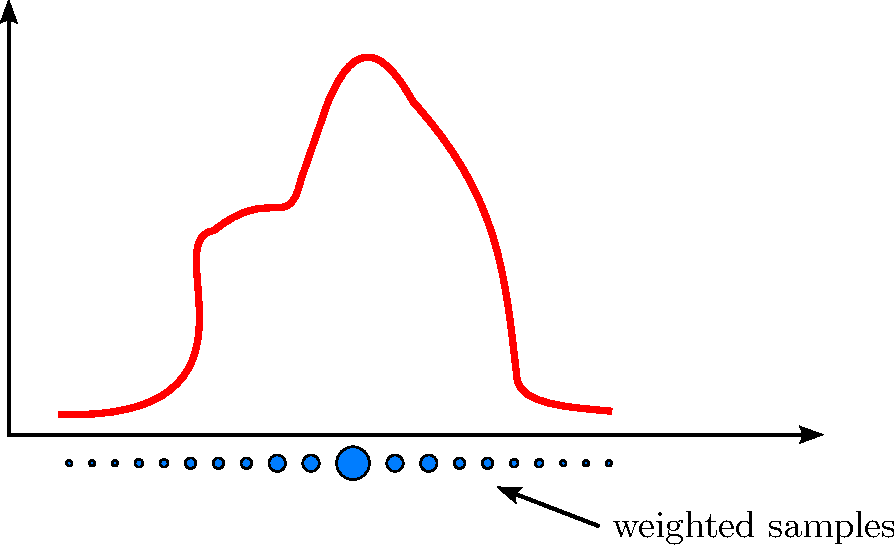
\includegraphics[width=0.4\columnwidth]{./images/particle_filter/arbitrary_distribution_weighted_samples.pdf}
    \end{center}
\end{frame}

\begin{frame}
    \frametitle{Particle Filter}
    \note{Content from Cyrill Stachniss's video: https://youtu.be/MsYlueVDLI0}
    \footnotesize
    \begin{itemize}
        \item Note that this is an approximation of the PDF (\emph{Probabilistic Density Function})
        \item It is important to have a sufficient number of samples to be able to adequately represent the PDF.
    \end{itemize}
\end{frame}

\begin{frame}
    \frametitle{Particle Ensemble}
    \note{Information taken from Cyrill Stachniss's video https://youtu.be/MsYlueVDLI0}
    
    \begin{itemize}
        \item Weighted Particle Ensemble
        
        \begin{center}
            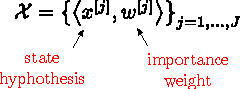
\includegraphics[width=0.5\columnwidth]{./images/particle_filter/weighted_samples.pdf}
        \end{center}
        
        \item The particles represent the posterior belief given by
            \begin{equation*}
                p(x) = \sum_{j=1}^{J} w^{[j]} \delta_{x^{[j]}}(x)
            \end{equation*}
            where $\delta_{x^{[j]}}(x)$ is the Dirac function centered at the location of particle $x^{[j]}$.
            
            \begin{equation*}
                \delta(y) =
                \begin{cases}
                \infty, & y = x^{[j]} \\
                0, & y \neq x^{[j]}
                \end{cases};
            \end{equation*}
        
            \note{The Dirac function simulates impulses or events}
            \note{The Dirac function tends to infinity when $x=j$ and, for any other value of $x$, it is equal to 0.}
            
            \note{We will need a greater number of particles the more complex the pdf is}
    
    \end{itemize}
    
\end{frame}

\begin{frame}
    \frametitle{Particles for Approximation}
    \note{Content from Cyrill Stachniss's video: https://youtu.be/MsYlueVDLI0}
    
    \begin{itemize}
        \item Particles approximating a function
        
        \begin{center}
            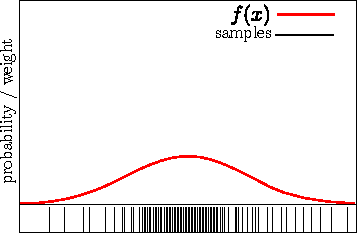
\includegraphics[width=0.45\columnwidth]{./images/particle_filter/gaussian_approximation_by_sampling.pdf}
            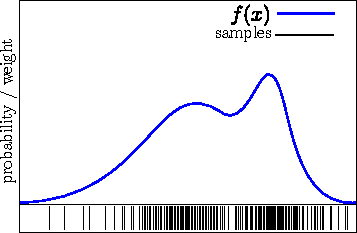
\includegraphics[width=0.45\columnwidth]{./images/particle_filter/particles_for_approximation.pdf}
        \end{center}

        \item More particles in a region indicates higher probability
    \end{itemize}
    
    \begin{center}
        \alert{How to obtain these samples?}
    \end{center}

    \note{Closed-form sampling is only possible for few distributions}
\end{frame}

\begin{frame}
    \frametitle{Closed-Form Sampling is Only Possible for Few Distributions}
    \note{Content from Cyrill Stachniss's video: https://youtu.be/MsYlueVDLI0}

    \begin{itemize}
        \item Example: Sampling from a Gaussian Distribution
    \end{itemize}

    \begin{figure}
        \begin{minipage}[m]{.5\textwidth}
            \raggedright
            \begin{center}
                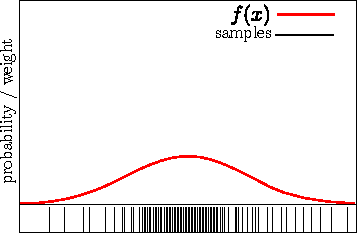
\includegraphics[width=\columnwidth]{./images/particle_filter/gaussian_approximation_by_sampling.pdf}
            \end{center}
        \end{minipage}%
        \begin{minipage}[m]{.5\textwidth}
            \raggedleft
            \centering
            \begin{equation*}
                x \leftarrow \frac{1}{2} \sum_{i=1}^{12} \text{rand}(-\sigma, \sigma)    
            \end{equation*}
        \end{minipage}
    \end{figure}

    How to sample using other distributions?

    \note{Rejection sampling technique. Not used in particle filters because it is a very inefficient technique.}

    \note{Importance Sampling Principle Technique}
\end{frame}

\begin{frame}
    \frametitle{Importance Sampling Principle}
    \note{Information taken from Cyrill Stachniss's video https://youtu.be/MsYlueVDLI0}
    
    \scriptsize
    
    \begin{itemize}
        \item We can use a different distribution $\pi$ to generate samples from a distribution $f$ (the one we actually want to use for sampling)
        \item Consider the ``differences between $\pi$ and $f$'' using a weight $w = f(x) / \pi(x)$
        \item Target Distribution Function (\emph{target}) $f$
        \item Proposed Distribution Function (\emph{Proposal}) $\pi$
        \item Precondition:
        $f(x) > 0 \implies \pi(x) > 0$
        
        \note{The precondition is required since if there is a case where f(x) > 0 and pi(x) < 0 means that there is zero probability of generating that sample with the function pi (proposal), and therefore we will never be able to generate a sample for f (target). We cannot adequately approximate f. Furthermore, it can be seen that for the calculation of the weights w, if pi(x) = 0, then we would have an undefined (infinite) weight, which is not what we want.}

        \begin{center}
            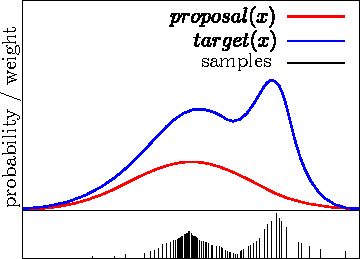
\includegraphics[width=0.4\textwidth]{./images/particle_filter/importance_sampling_principle.pdf}
        \end{center}

        The greater the difference between the value of the $target$ function and the $proposal$ function, the more weight is assigned to the sample (higher bars). Note that the proposal function determines the frequency of the samples. In this case, for the highest part of the target function, there are few samples, but they have a high weight.
    
    \end{itemize}
    
    \note{The Importance Sampling Principle tells us that we can use a proposal distribution to generate samples from a target distribution (the one we actually want to sample from), compensating for any errors we make. Errors here mean the difference between the value of the red curve and the blue curve. To do this, we must be able to evaluate the proposal function and the target function for the same input and calculate the weight w. The weights are used to compensate.}
\end{frame}


\begin{frame}
    \frametitle{Particle Filter for Dynamic State Estimation Problems}
    \note{Information taken from the video by Cyrill Stachniss https://youtu.be/MsYlueVDLI0}
    
    \begin{itemize}
        \item PF implements a Recursive Bayesian Filter (performs a Prediction step and a Correction step)
        \item Nonparametric approach (allows working with non-Gaussian distributions)
        \item Models the distribution using samples
        \item \textbf{Prediction}: extract from the \emph{proposal} distribution
        \item \textbf{Correction}: weighting with the ratio between the \emph{target} and the \emph{proposal} distribution
        \item \alert{The more samples we use, the better the estimate!}
    \end{itemize}
\end{frame}

\begin{frame}
    \frametitle{Particle Filter Algorithm}
    \note{Information taken from Cyrill Stachniss's video https://youtu.be/MsYlueVDLI0}
    
    \begin{enumerate}
        \item Sample the particles using the \emph{proposal} distribution.
            \begin{equation*}
                x_{t}^{[j]} \sim proposal(x_{t} | \ldots) \qquad \text{(analogous to sampling the red curve)}
            \end{equation*}
        \item Calculate the importance weights
            \begin{equation*}
                w_t^{[j]} = \frac{target(x_t^{[j]})}{proposal(x_t^{[j]})} \qquad \text{{(weights to compensate for the differences between \emph{proposal} and \emph{target})}}
            \end{equation*}
        \item Resampling: Take particle $i$ with probability $w_{t}^{[j]}$ and repeat $J$ times.
            \note{Note that in resampling we are replacing the weight of a sample by the frequency of this sample. That is, the more weight a sample has, the more often we will choose it.}
            
            \note{Also, in resampling, by choosing samples with greater weight and not choosing samples with less weight, we are better describing the probability distribution mass since particles with less weight do not contribute much to the probability distribution mass, and this allows for better use of the computer's memory.}
            
            (that is, we generate compensating samples)
    \end{enumerate}
    \note{Replacing unlikely samples with more likely ones}
    
    \vspace{1cm}
    
    Interpreting PF with the Recursive Bayes Filter:
    \begin{itemize}
        \item Step 1 corresponds to the Prediction Step using the motion model, and
        \item Steps 2 and 3 correspond to the Correction Step using the observation model to calculate the weights.
    \end{itemize}
    
\end{frame}

\begin{frame}
    \frametitle{Particle Filter Algorithm}
    \note{Content from Cyrill Stachniss's video: https://youtu.be/MsYlueVDLI0}

    \begin{algorithmic}[1]
    \Procedure{ParticleFilter}{$\mathcal{X}_{t-1}, u_{t}, z_{t}$}
    \State $\bar{\mathcal{X}}_t = \mathcal{X}_t = \emptyset$
    \For{$j = 1$ to $J$}
        \State sample $x_t^{[j]} \sim \pi(x_t)$
        \State $w_t^{[j]} = \dfrac{p(x_t^{[j]})}{\pi(x_t^{[j]})}$
        \State $\bar{\mathcal{X}}_t = \bar{\mathcal{X}}_t + \langle x_t^{[j]}, w_t^{[j]}\rangle$
    \EndFor
    \For{$j = 1$ to $M$}
        \State Draw $i$ with probability $\propto w_t^{[i]}$
        \State Add $x_t^{[i]}$ to $\mathcal{X}_t$
    \EndFor
    \State return $\mathcal{X}_t$
    \EndProcedure
    \end{algorithmic}
\end{frame}

\begin{frame}
    \frametitle{Monte Carlo Localization}
    \note{Content from Cyrill Stachniss's video: https://youtu.be/MsYlueVDLI0}

    Monte Carlo Localization: Particle Filter for robot localization.
\end{frame}

\begin{frame}
    \frametitle{Monte Carlo Localization}
    \note{Information taken from Cyrill Stachniss's video https://youtu.be/MsYlueVDLI0}
    
    \begin{itemize}
        \item Each particle is a pose hypothesis
        \item \emph{Proposal} is the motion model
            \begin{equation*}
                \state_t^{[j]} \sim p(\state_{t} \, | \, \state_{t-1}, \controlCommand_{t})
            \end{equation*}
        
            Here, we sample from the \emph{proposal} distribution $p(\state_{t} \, | \, \state_{t-1}, \controlCommand_{t})$. Note that since $\controlCommand_{t}$ is noisy, each particle moves with a certain degree of variance. For example, if $\controlCommand_{t}$ says the robot moved \SI{1}{\meter} then there will be one particle moving \SI{0.97}{\meter}, another \SI{1.02}{\meter}, etc.
        
        \item Correction via the observation model
            \begin{equation*}
                w_t^{[j]} = \frac{target}{proposal} \propto p(z_t \, | \, x_t, m)
            \end{equation*}
        \note{it is proportional because we normalized the weights so that their sum is 1.}
    \end{itemize}
\end{frame}

\begin{frame} 
    \frametitle{Particle Filter for Localization} 
    \note{Information taken from Cyrill Stachniss Video https://youtu.be/MsYlueVDLI0} 
    
    \begin{algorithmic}[1] 
        \Procedure{ParticleFilter}{$\mathcal{X}_{t-1}, u_{t}, z_{t}$} 
        \State $\bar{\mathcal{X}}_t = \mathcal{X}_t = \emptyset$ 
        \For{$j = 1$ to $J$} 
        \State Sample \alert{$x_t^{[j]} \sim p(x_t \, | \, u_t, x_{t-1}^{[j]})$} 
        \State $w_t^{[j]} = \alert{p(z_t \, | \, x_t^{[j]})}$ 
        \State $\bar{\mathcal{X}}_t = \bar{\mathcal{X}}_t + \langle x_t^{[j]}, w_t^{[j]}\rangle$ 
        \EndFor 
        \For{$i = 1$ to $J$} 
        \State Draw $i \in 1,\ldots,J$ with probability $\propto w_t^{[i]}$ 
        \State Add $x_t^{[i]}$ to $\mathcal{X}_t$ 
        \EndFor 
        \State return $\mathcal{X}_t$ 
        \EndProcedure 
    \end{algorithmic}
\end{frame}

\begin{frame}
    \frametitle{Monte Carlo Localization - Correction Step}
    \note{Information taken from Cyrill Stachniss's video https://youtu.be/MsYlueVDLI0}
    
    \begin{center}
        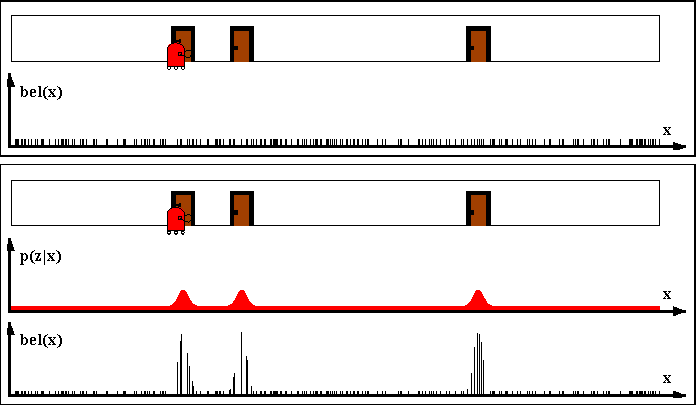
\includegraphics[width=0.8\textwidth]{./images/particle_filter/monte_carlo_correction.pdf}
    \end{center}
    
\end{frame}
    
\begin{frame}
    \frametitle{Monte Carlo Localization - Resampling and Prediction}
    \note{Information taken from Cyrill Stachniss's video https://youtu.be/MsYlueVDLI0}
    
    \begin{center}
        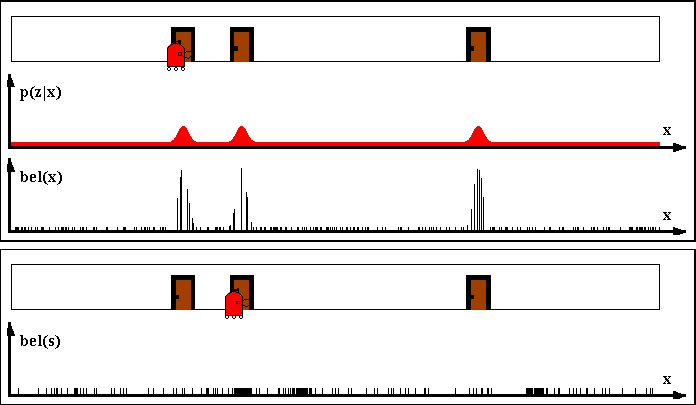
\includegraphics[width=0.8\textwidth]{./images/particle_filter/monte_carlo_resample_and_predict.pdf}
    \end{center}
    
\end{frame}
    
\begin{frame}
    \frametitle{Monte Carlo Localization - Correction Step 2}
    \note{Information taken from Cyrill Stachniss's video https://youtu.be/MsYlueVDLI0}
    
    \begin{center}
        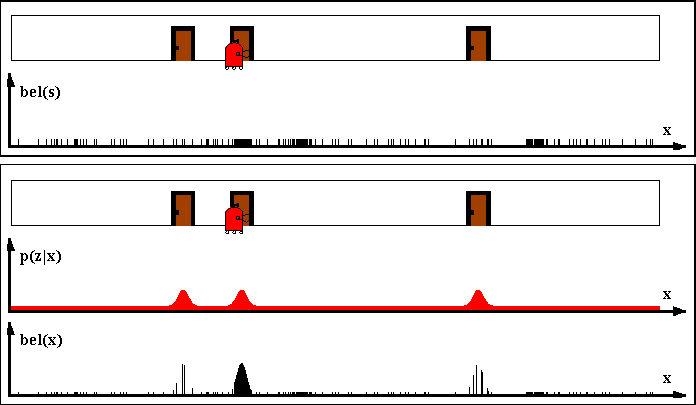
\includegraphics[width=0.8\textwidth]{./images/particle_filter/monte_carlo_correction2.pdf}
    \end{center}
    
\end{frame}
    
\begin{frame}
    \frametitle{Monte Carlo Localization - Resampling and Prediction 2}
    \note{Information taken from Cyrill Stachniss's video https://youtu.be/MsYlueVDLI0}
    
    \begin{center} 
        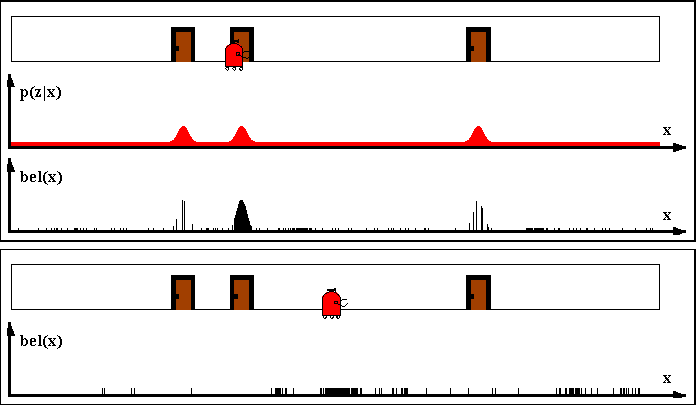
\includegraphics[width=0.8\textwidth]{./images/particle_filter/monte_carlo_resample_and_predict2.pdf} 
    \end{center}
    
\end{frame}

\begin{frame}
    \frametitle{Resampling}
    \note{Content from Cyrill Stachniss's video: https://youtu.be/MsYlueVDLI0}

    \begin{itemize}
        \item Take particle $i$ with probability $w_t^{[i]}$. Repeat $J$ times.
        \item Informally: ``Replace unlikely samples with more likely ones''
        \item Survival of the fittest
        \item ``Trick'' to prevent many samples from covering unlikely states
        \item Necessary, since we have a limited number of samples (finite memory)
    \end{itemize}
\end{frame}

\begin{frame}
    \frametitle{Resampling Methods}
    \note{Content from Cyrill Stachniss's video: https://youtu.be/MsYlueVDLI0}

    \scriptsize

    \only<1>{
        \begin{center}
            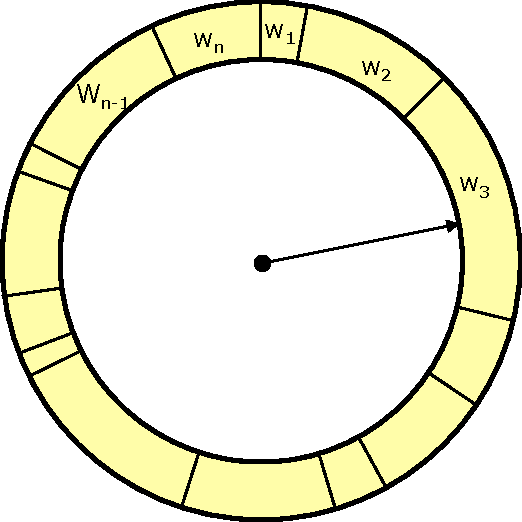
\includegraphics[width=0.3\textwidth]{./images/particle_filter/resampling_rulette_wheel1.pdf}
        \end{center}
    }
    \only<2>{
        \begin{center}
            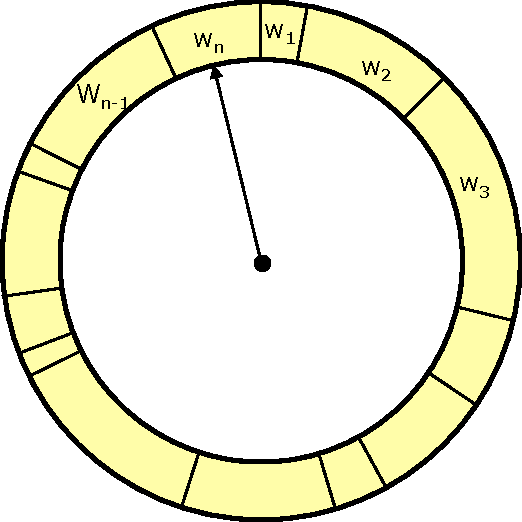
\includegraphics[width=0.3\textwidth]{./images/particle_filter/resampling_rulette_wheel2.pdf}
        \end{center}
    }
    \only<3>{
        \begin{center}
            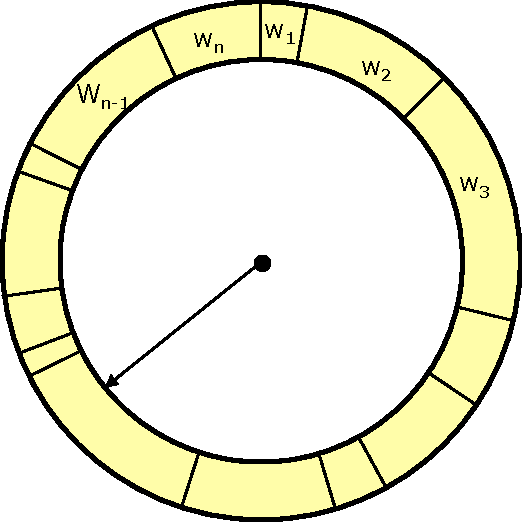
\includegraphics[width=0.3\textwidth]{./images/particle_filter/resampling_rulette_wheel3.pdf}
        \end{center}
    }
    \begin{itemize}
        \item Roulette Wheel
        \item The roulette wheel's buckets represent the weights of the particles. The larger the bucket, the more likely it is that the particle will be selected.
        \item We have to do this $J$ times. We have to find where the ball lands. We can do this with binary search. The sum of all the roulette wheel's weights is 1. If we roll a random number between 0 and 1, then with binary search we can find out which bucket it lands in.
        \item Binary search to find out which bucket the ball lands in ($O(J \log(J))$)
    \end{itemize}
\end{frame}

\begin{frame}
    \frametitle{Resampling Methods}
    \note{Content from Cyrill Stachniss's video: https://youtu.be/MsYlueVDLI0}

    \footnotesize

    \only<1>{
        \begin{center}
            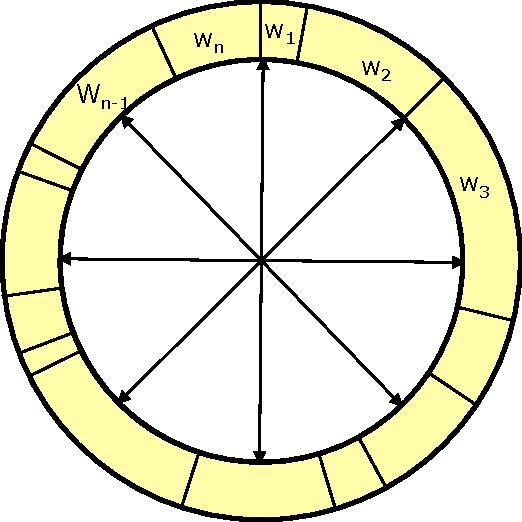
\includegraphics[width=0.3\textwidth]{./images/particle_filter/resampling_stochastic_universal_sampling1.pdf}
        \end{center}
    }
    \only<2>{
        \begin{center}
            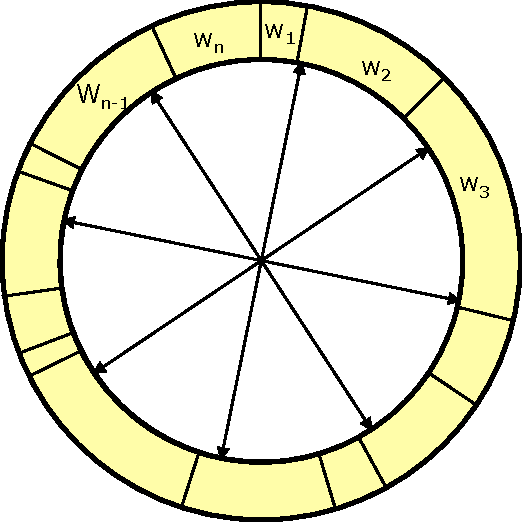
\includegraphics[width=0.3\textwidth]{./images/particle_filter/resampling_stochastic_universal_sampling2.pdf}
        \end{center}
    }

    \begin{itemize}
        \item Stochastic universal sampling (using $J$ equidistant arrows)
        \item Also called \emph{Low-Variance Resampling} (prevents particles from concentrating quickly)
        \item Using J arrows and equidistant them. We rotate them all together and select J particles. So when we roll a random number, all J particles are selected at once.
        \item Has a linear computational cost of $O(J)$ because we only have to iterate through the weights once to see where all the arrows fall.
    \end{itemize}

    \note{Example 8 arrows 45 degrees apart from each other.}
\end{frame}

\begin{frame}
    \frametitle{Resampling}
    \note{Information taken from Cyrill Stachniss's video https://youtu.be/MsYlueVDLI0}
    
    \begin{itemize}
        \item Sampling with replacement (we sample by taking a particle and then placing it back in the bag)
        \item Roulette Wheel resampling is easy to understand but suboptimal in practice
        \item \alert{What happens if all the particles have the same weight?}
        \note{If all the particles have the same weight, it would be like having a sensor that gives me no information.}
        \note{If all the particles have the same weight, resampling will randomly select particles and duplicate them, and other particles will not be selected and will die. And this happens without one particle being better than another. This leads the system to converge at any location.} 
        \note{Therefore, if all the particles have the same weight then it does not make sense to choose one over the other.} 
        
        \note{ 
        https://robotics.stackexchange.com/questions/16093/why-does-the-low-variance-resampling-algorithm-for-particle-filters-work 
        
        TLDR; A particle filter’s convergence rate is inversely proportional to the variance in the parents’ offspring counts. Low variance means fast convergence. 
        
        NOTE: Below, I discuss (but never explicitly mention) the concept of variance effective population size. 
        
        The effectiveness of this resampling strategy makes a lot of sense when you consider that the particle filter is, at its core, an evolutionary algorithm (EA). All EAs tend to lose diversity because of the random sampling step, at a rate proportional to the variance in how many offspring the parents produce. This effect is known as genetic drift, and it adversely affects biological populations as well. As a result of this diversity loss, the EA prematurely converges to suboptimal solutions. This is bad news. 
        
        Intuitively, genetic drift makes sense. When parents are chosen at random (the most common setup), those with low fitness/quality are likely to get skipped and produce zero offspring and be eliminated from the gene pool, thus reducing the population's diversity. Now, the rate at which natural selection improves a population's fitness is directly proportional to the population's diversity—diversity is literally the fuel that drives natural selection. Genetic drift reduces the diversity, thus decreasing the rate at which the population's fitness can improve and causing the aforementioned bad news. 
        
        Let's now look at the low-variance resampling method. This method gives almost every parent exactly the number of offspring that they would be expected to obtain with the random sampling, without the extra uncertainty (variance). This reduces genetic drift and greatly increases the efficiency with which the particle filter can improve its solution and/or adapt to changing conditions 
        } 
        
    \end{itemize}
\end{frame}

\begin{frame} 
    \frametitle{Low Variance Resampling Idea} 
    \note{Information taken from Cyrill Stachniss Video https://youtu.be/MsYlueVDLI0} 
    
    \begin{center} 
        \only<1>{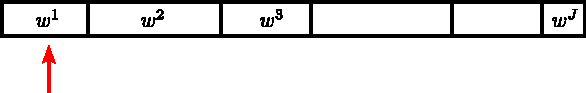
\includegraphics[width=0.7\textwidth]{./images/particle_filter/low_variance_resampling1.pdf}} 
        \only<2>{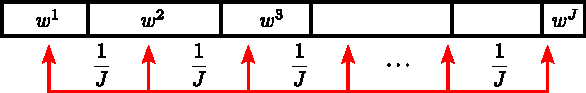
\includegraphics[width=0.7\textwidth]{./images/particle_filter/low_variance_resampling2.pdf}} 
    \end{center} 
    
    \begin{enumerate} 
        \item<1-> We take a random value $r$ between 0 and $\dfrac{1}{j}$ 
        \item<2> We take $J-1$ particles in $\dfrac{1}{J}$ steps (based on accumulated weight) 
    \end{enumerate}
    
\end{frame}

\begin{frame} 
    \frametitle{Low Variance Resampling: Efficient Implementation} 
    \note{Information taken from Cyrill Stachniss Video https://youtu.be/MsYlueVDLI0} 
    
    \begin{center} 
        \only<1>{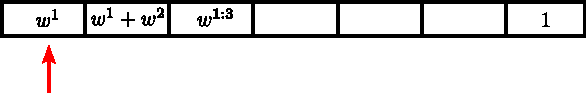
\includegraphics[width=0.7\textwidth]{./images/particle_filter/low_variance_resampling_efficient_implementation1.pdf}} 
        \only<2>{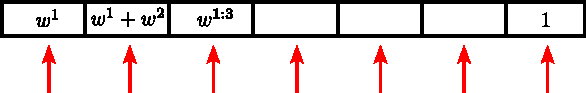
\includegraphics[width=0.7\textwidth]{./images/particle_filter/low_variance_resampling_efficient_implementation2.pdf}} 
    \end{center} 
    
    \begin{enumerate} 
        \item<1-> We take a random value $r$ between 0 and $\dfrac{1}{j}$ 
        \item<2> 
        \begin{algorithmic}[1] 
            \For{$j = 1$ to $J$} 
            \State $U = r + (j - 1) \dfrac{1}{J}$ 
            \While{$\left(U > cum[i]\right)$} 
            \State $i++$ 
            \EndWhile 
            \State Add $x_t^{[i]}$ to $\bar{\mathcal{X}}_t$ 
            \EndFor 
        \end{algorithmic} 
        % \begin{fleqn}[\parindent] 
        % \begin{align*} 
        % for &(j=1 \dots J)\\ 
        % &U = r + j \dfrac{1}{J}\\ 
        % &while (U > cum[i]) \quad i++;\\ 
        % &pick\_particle(i) 
        % \end{align*} 
        % \end{fleqn} 
    \end{enumerate}
    
\end{frame}


\begin{frame}
    \frametitle{Low Variance Resampling}
    \begin{algorithmic}[1]
        \Procedure{LowVarianceResampling}{$\mathcal{X}_{t}$, $\mathcal{W}_{t}$}
        \State $\bar{\mathcal{X}}_t = \emptyset$
        \State $r = \text{rand}(0; J^{-1})$
        \State $c = w_t^{[1]}$
        \State $i = 1$
        \For{$j = 1$ to $J$}
            \State $U = r + (j - 1) J^{-1}$
            \While{$U > c$}
                \State $i = i + 1$
                \State $c = c + w_t^{[i]}$
            \EndWhile
            \State Add $x_t^{[i]}$ to $\bar{\mathcal{X}}_t$
        \EndFor
        \State Return $\bar{\mathcal{X}}_t$
        \EndProcedure
    \end{algorithmic}
\end{frame}

\begin{frame}
    \frametitle{Low Variance Resampling}
    \note{Information taken from Cyrill Stachniss's video https://youtu.be/MsYlueVDLI0}
    
    \begin{itemize}
        \item Performs resampling that keeps samples if they have equal weights.
        \item It's faster than roulette wheel resampling: $O(J)$ vs. $O(J \log J)$
        \item \alert{We will always use Low Variance Resampling!}
    \end{itemize}
\end{frame}

\begin{frame}
    \frametitle{Disadvantages of Particle Filter}
    \note{Information taken from Cyrill Stachniss's video https://youtu.be/MsYlueVDLI0}
    
    \begin{itemize}
        \item Does not scale well for high-dimensional spaces
        \note{PF becomes very computationally expensive since we will need many particles to cover the probability distribution. PF works well for low dimensions; up to 4 is possible, but more requires adopting certain heuristics to reduce the number of particles and ensure they are representative.}
        \note{The number of particles grows exponentially with the dimensions of the state}
        \item Problematic in situations with high uncertainty
        \item \emph{Depletion Problem} (most particles have low weights)
        \note{The Depletion Problem: occurs when we have very few particles compared to the dimensionality of the state. The particles do not cover the areas of highest probability and therefore die, causing the filter to eventually diverge.
        Example: Imagine you have 100 particles tracking the position of a robot. If the robot makes a sharp turn, many particles will have low weights because they do not predict the movement well. After resampling, only a few particles will "survive," and the filter will lose diversity, affecting future estimates.}
    \end{itemize}
\end{frame}

\begin{frame}
    \frametitle{Advantages}
    \note{Information taken from Cyrill Stachniss's video https://youtu.be/MsYlueVDLI0}
    
    \begin{itemize}
        \item Can work with non-Gaussian distributions
        \item Works well in low-dimensional spaces
        \item Can handle ambiguities in data associations. \note{We can make each particle have its own way of associating data. Since there is no uncertainty associated with this, we can make decisions dependent on each particle and see which survives.}
        \item Can easily incorporate different sensing modalities \note{We can incorporate different sensing modalities by simply multiplying the weight with the computed weight of another sensor}
        \item Robust \note{Robust because even when the models are not perfect, it will be able to compute good beliefs}
        \item Easy to implement
    \end{itemize}
\end{frame}
    
\begin{frame}
    \frametitle{Summary – Particle Filter}
    \note{Information taken from Cyrill Stachniss's video https://youtu.be/MsYlueVDLI0}
    
    \begin{itemize}
        \item Particle filters are recursive, non-parametric Bayesian filters
        \item The Posterior Belief is represented by an ensemble of weighted samples
        \item Not limited to Distributions Gaussians
        \item Proposal for extracting samples at $t+1$
        \item Weight to account for differences between the proposal and the target
        \item The art lies in designing appropriate motion and sensing models
    \end{itemize}
\end{frame}
    
\begin{frame}
    \frametitle{Summary – Localization with PF}
    \note{Information taken from Cyrill Stachniss's video https://youtu.be/MsYlueVDLI0}
    
    \begin{itemize}
        \item Particles propagate according to the motion model
        \item They are weighted according to the probability of the observation
        \item This is called Monte Carlo Localization (MCL)
        \item MCL is a gold standard for localizing mobile robots in \emph{indoor} environments
    \end{itemize}
\end{frame}